\section{Problem Formulation}\label{sec:formulation}

\subsection{Alpha Factor}

We consider a stock market with $n$ stocks in a period of $T$ trading days in total. On each trading day $t \in \braces{1, 2, \cdots, T}$, each stock $i$ corresponds to a feature vector $x_{ti} \in \mathbb{R}^{m\tau}$, comprised of $m$ raw features such as opening/closing price in the recent $\tau$ days\footnote{This ``unrolling'' of historical data introduces redundancy. Namely, feature vectors of a stock on consecutive trading days have overlapping sections. This notation is chosen for the convenience of demonstration.}. Finally, we define an \emph{alpha factor} $f$ as a function mapping feature vectors of all stocks on a trading day $X \in \mathbb{R}^{n\times m\tau}$ into \emph{alpha values} $z = f(X) \in \mathbb{R}^n$. We will use the word ``alpha'' for both an alpha factor and its corresponding values in the following sections.

\subsection{Alpha Factor Mining}

To measure the effectiveness of an alpha, we calculate the information coefficient (IC) between the true stock trend it aims to predict $y_t \in \mathbb{R}^n$ and the factor values $f(X_t)$. We denote the daily IC function as $\sigma: \mathbb{R}^{n} \times \mathbb{R}^{n} \to [-1, 1]$, which is defined as the Pearson's correlation coefficient:
\begin{equation}
    \sigma(u_t, v_t) = \frac{\sum_{i=1}^{n} (u_{ti} - \bar{u}_t)(v_{ti} - \bar{v}_t)}{\sqrt{\sum_{i=1}^{n} (u_{ti} - \bar{u_t})^2 \sum_{i=1}^{n} (v_{ti} - \bar{v_t})^2}}.
    \label{eq:pearson}
\end{equation}
Such value can be calculated on every trading day between an alpha and the prediction target. For convenience, we denote the IC values between two sets of vectors averaged over all trading days as $\bar{\sigma}(u, v) = \expectation{t}{\sigma(u_t, v_t)}$.

We use the average IC between an alpha and the return to measure the effectiveness of an alpha factor on a stock trend series $y = \braces{y_1, y_2, \cdots, y_T}$:
\begin{equation}
    \bar{\sigma}_y(f) = \bar{\sigma}(f(X), y).
\end{equation}

As mentioned above, the output of a combination model can be seen as a ``mega-alpha'', mapping raw inputs into alpha values. Therefore, we denote the combination model as $c(X;\mathcal{F},\theta)$, where $\mathcal{F} = \braces{f_1, f_2, \cdots, f_k}$ is a set of alphas to combine, and $\theta$ denotes the parameters of the combination model. We would like the combination model to be optimal w.r.t. a given alpha set $\mathcal{F}$ on the training dataset $y$, that is:

\begin{equation}
    \begin{aligned}
        c^*(X; \mathcal{F}) & = c(X; \mathcal{F}, \theta^*), \quad \textrm{where} \\
        \theta^* & = \argmax_\theta \bar{\sigma}_y(c(\cdot; \mathcal{F}, \theta)).
    \end{aligned}
\end{equation}

Conclusively, the task of mining a set of alphas can be defined as the optimization problem $\argmax_\mathcal{F} c^*(\cdot; \mathcal{F})$.

\begin{figure}[t]
    \centering
    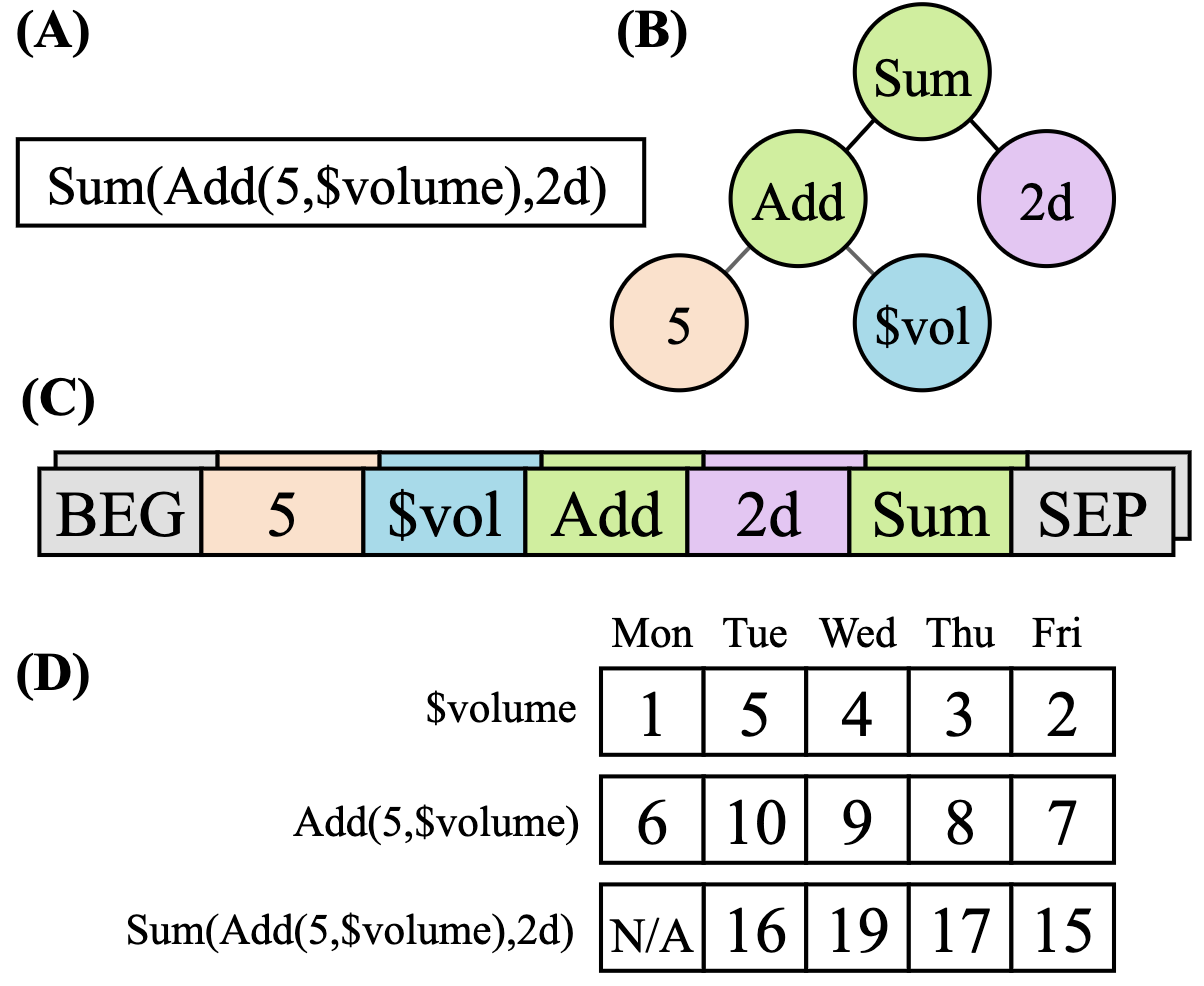
\includegraphics[width=0.7\linewidth]{Images/formulation.png}
    \caption{(A) An example of a formulaic alpha. (B) Its equivalent expression tree. (C) Its reverse Polish notation (RPN). Note that \emph{BEG} and \emph{SEP} are sequence indicators later mentioned in our framework. (D). Step-by-step computation of this alpha on an example time series.}
    \label{fig:formulation}
\end{figure}

\subsection{Formulaic Alpha}

Formulaic alphas are expressed as mathematical expressions, consisting of various operators and the raw input features mentioned before. Some examples of the operators are the elementary functions (like ``$+$'' and ``$\log$'') operated on one-day data, called cross-section operators, and operators that require data from a series of days, called time-series operators (e.g. ``Min(close, 5)'' gives the lowest closing price of a stock in the recent 5 days). A list of all the operators used in our framework is given in Appendix \ref{sec:ops}.

Such formulas can be naturally represented by an expression tree, with each non-leaf node representing an operator, and children of a node representing the operands. To generate such an expression, our model represents the expression tree by its postorder traverse, with the children's order also defined by the traversing order. In other words, the model represents a formula as its reverse Polish notation (RPN). It is easy to see that such notation is unambiguous since the arities of the operators are all known constants. See Figure \ref{fig:formulation} for an example of a formulaic alpha expression together with its corresponding tree and RPN representations.
